
%--------------------------------------
%ELECTROTECHNIQUE - SCHEMA DE LIAISON A LA TERRE
%--------------------------------------

%utiliser les environnement \begin{comment} \end{comment} pour mettre en commentaire le préambule une fois la programmation appelée dans le document maître (!ne pas oublier de mettre en commentaire \end{document}!)

\begin{comment}

\documentclass[a4paper, 11pt, twoside, fleqn]{memoir}

\usepackage{AOCDTF}

\marqueurchapitre

%lien d'édition des figures Tikz sur le site mathcha.io (rajouter le lien d'une modification effectuée sur la figure tikz avec le nom du modificateur car il n'y a qu'un lien par compte)

%lien éditeur Bruno Douchy : https://www.mathcha.io/editor/r4VYjhyjSEpUxKMwljHvQeVj8fEKjQMvCGNknrl

%--------------------------------------
%corps du document
%--------------------------------------

\begin{document} %corps du document
	\openleft %début de chapitre à gauche

\end{comment}

\begin{figure}
\caption{Répartition des volumes dans une salle d'eau sans receveur}
\tikzset{every picture/.style={line width=0.5pt}} %set default line width to 0.75pt        

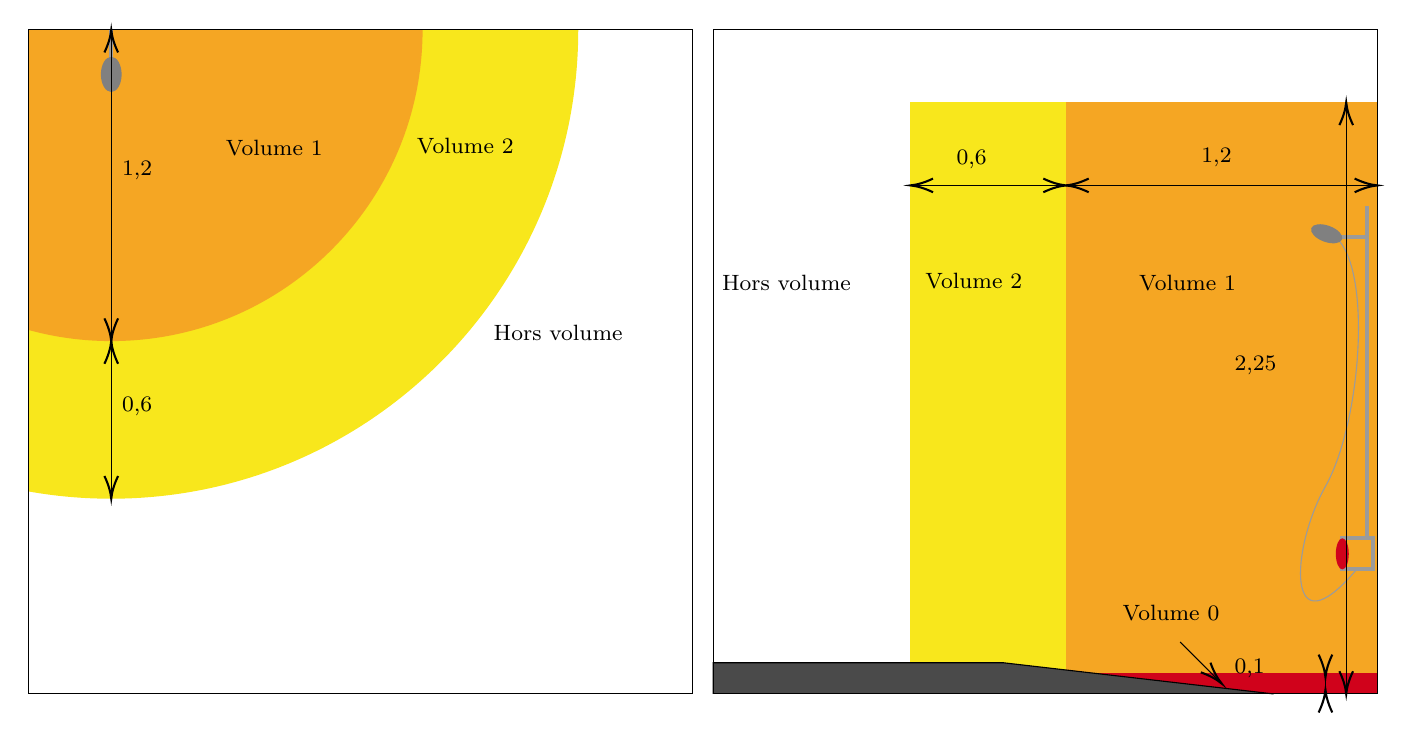
\begin{tikzpicture}[x=0.75pt,y=0.75pt,yscale=-1,xscale=1]
%uncomment if require: \path (0,550); %set diagram left start at 0, and has height of 550

%Shape: Rectangle [id:dp662524575372376] 
\draw  [draw opacity=0][fill={rgb, 255:red, 245; green, 166; blue, 35 }  ,fill opacity=1 ] (505,75) -- (655,75) -- (655,360) -- (505,360) -- cycle ;
%Shape: Path Data [id:dp8475067670718847] 
\draw  [draw opacity=0][fill={rgb, 255:red, 248; green, 231; blue, 28 }  ,fill opacity=1 ] (44.86,265.94) .. controls (31.26,265.94) and (17.94,264.73) .. (5,262.41) -- (5,40) -- (270,40) .. controls (270,164.78) and (169.2,265.94) .. (44.86,265.94) -- cycle ;
%Shape: Path Data [id:dp6391722198147811] 
\draw  [draw opacity=0][fill={rgb, 255:red, 245; green, 166; blue, 35 }  ,fill opacity=1 ] (45,190) .. controls (31.15,190) and (17.73,188.12) .. (5,184.61) -- (5,40) -- (195,40) .. controls (195,122.84) and (127.84,190) .. (45,190) -- cycle ;
%Straight Lines [id:da30342442827537275] 
\draw    (45,192) -- (45,263.94) ;
\draw [shift={(45,265.94)}, rotate = 270] [color={rgb, 255:red, 0; green, 0; blue, 0 }  ][line width=0.75]    (10.93,-3.29) .. controls (6.95,-1.4) and (3.31,-0.3) .. (0,0) .. controls (3.31,0.3) and (6.95,1.4) .. (10.93,3.29)   ;
\draw [shift={(45,190)}, rotate = 90] [color={rgb, 255:red, 0; green, 0; blue, 0 }  ][line width=0.75]    (10.93,-3.29) .. controls (6.95,-1.4) and (3.31,-0.3) .. (0,0) .. controls (3.31,0.3) and (6.95,1.4) .. (10.93,3.29)   ;
%Shape: Ellipse [id:dp9403307541201106] 
\draw  [draw opacity=0][fill={rgb, 255:red, 128; green, 128; blue, 128 }  ,fill opacity=1 ] (40,61.5) .. controls (40,56.81) and (42.24,53) .. (45,53) .. controls (47.76,53) and (50,56.81) .. (50,61.5) .. controls (50,66.19) and (47.76,70) .. (45,70) .. controls (42.24,70) and (40,66.19) .. (40,61.5) -- cycle ;
%Straight Lines [id:da02087532483936594] 
\draw [color={rgb, 255:red, 155; green, 155; blue, 155 }  ,draw opacity=1 ][line width=1.5]    (635,140) -- (650,140) -- (650,125) -- (650,285) ;
%Shape: Rectangle [id:dp8026516698473696] 
\draw  [color={rgb, 255:red, 155; green, 155; blue, 155 }  ,draw opacity=1 ][line width=1.5]  (638,285) -- (653,285) -- (653,300) -- (638,300) -- cycle ;
%Shape: Ellipse [id:dp5617322251469574] 
\draw  [draw opacity=0][fill={rgb, 255:red, 208; green, 2; blue, 27 }  ,fill opacity=1 ] (635,292.5) .. controls (635,288.36) and (636.4,285) .. (638.12,285) .. controls (639.84,285) and (641.24,288.36) .. (641.24,292.5) .. controls (641.24,296.64) and (639.84,300) .. (638.12,300) .. controls (636.4,300) and (635,296.64) .. (635,292.5) -- cycle ;
%Curve Lines [id:da34152496146470934] 
\draw [color={rgb, 255:red, 155; green, 155; blue, 155 }  ,draw opacity=1 ]   (645,300) .. controls (610.74,340.76) and (613,290.13) .. (630,260) .. controls (647,229.87) and (652.89,156) .. (635,140) ;
%Straight Lines [id:da3291709567122535] 
\draw    (507,115) -- (653,115) ;
\draw [shift={(655,115)}, rotate = 180] [color={rgb, 255:red, 0; green, 0; blue, 0 }  ][line width=0.75]    (10.93,-3.29) .. controls (6.95,-1.4) and (3.31,-0.3) .. (0,0) .. controls (3.31,0.3) and (6.95,1.4) .. (10.93,3.29)   ;
\draw [shift={(505,115)}, rotate = 0] [color={rgb, 255:red, 0; green, 0; blue, 0 }  ][line width=0.75]    (10.93,-3.29) .. controls (6.95,-1.4) and (3.31,-0.3) .. (0,0) .. controls (3.31,0.3) and (6.95,1.4) .. (10.93,3.29)   ;
%Shape: Rectangle [id:dp3771388764567015] 
\draw  [draw opacity=0][fill={rgb, 255:red, 248; green, 231; blue, 28 }  ,fill opacity=1 ] (430,75) -- (505,75) -- (505,360) -- (430,360) -- cycle ;
%Shape: Ellipse [id:dp2508485797626314] 
\draw  [draw opacity=0][fill={rgb, 255:red, 128; green, 128; blue, 128 }  ,fill opacity=1 ] (629.22,142.02) .. controls (625.12,140.53) and (622.4,137.65) .. (623.15,135.59) .. controls (623.9,133.54) and (627.83,133.08) .. (631.93,134.57) .. controls (636.03,136.06) and (638.75,138.94) .. (638,141) .. controls (637.25,143.06) and (633.32,143.52) .. (629.22,142.02) -- cycle ;
%Straight Lines [id:da7753899978688642] 
\draw    (432,115) -- (503,115) ;
\draw [shift={(505,115)}, rotate = 180] [color={rgb, 255:red, 0; green, 0; blue, 0 }  ][line width=0.75]    (10.93,-3.29) .. controls (6.95,-1.4) and (3.31,-0.3) .. (0,0) .. controls (3.31,0.3) and (6.95,1.4) .. (10.93,3.29)   ;
\draw [shift={(430,115)}, rotate = 0] [color={rgb, 255:red, 0; green, 0; blue, 0 }  ][line width=0.75]    (10.93,-3.29) .. controls (6.95,-1.4) and (3.31,-0.3) .. (0,0) .. controls (3.31,0.3) and (6.95,1.4) .. (10.93,3.29)   ;
%Shape: Rectangle [id:dp5616018693868235] 
\draw  [draw opacity=0][fill={rgb, 255:red, 208; green, 2; blue, 27 }  ,fill opacity=1 ] (505,350) -- (655,350) -- (655,360) -- (505,360) -- cycle ;
%Straight Lines [id:da23151913869668295] 
\draw [fill={rgb, 255:red, 74; green, 74; blue, 74 }  ,fill opacity=1 ]   (335,360) -- (335,345) -- (475,345) -- (605,360) ;
%Shape: Square [id:dp20615639222385096] 
\draw   (335,40) -- (655,40) -- (655,360) -- (335,360) -- cycle ;
%Straight Lines [id:da4535884422765213] 
\draw    (640,77) -- (640,358) ;
\draw [shift={(640,360)}, rotate = 270] [color={rgb, 255:red, 0; green, 0; blue, 0 }  ][line width=0.75]    (10.93,-3.29) .. controls (6.95,-1.4) and (3.31,-0.3) .. (0,0) .. controls (3.31,0.3) and (6.95,1.4) .. (10.93,3.29)   ;
\draw [shift={(640,75)}, rotate = 90] [color={rgb, 255:red, 0; green, 0; blue, 0 }  ][line width=0.75]    (10.93,-3.29) .. controls (6.95,-1.4) and (3.31,-0.3) .. (0,0) .. controls (3.31,0.3) and (6.95,1.4) .. (10.93,3.29)   ;
%Straight Lines [id:da07910479855322938] 
\draw    (630,352) -- (630,358) ;
\draw [shift={(630,358)}, rotate = 90] [color={rgb, 255:red, 0; green, 0; blue, 0 }  ][line width=0.75]    (10.93,-3.29) .. controls (6.95,-1.4) and (3.31,-0.3) .. (0,0) .. controls (3.31,0.3) and (6.95,1.4) .. (10.93,3.29)   ;
\draw [shift={(630,352)}, rotate = 270] [color={rgb, 255:red, 0; green, 0; blue, 0 }  ][line width=0.75]    (10.93,-3.29) .. controls (6.95,-1.4) and (3.31,-0.3) .. (0,0) .. controls (3.31,0.3) and (6.95,1.4) .. (10.93,3.29)   ;
%Straight Lines [id:da2835004459782169] 
\draw [color={rgb, 255:red, 155; green, 155; blue, 155 }  ,draw opacity=1 ][line width=1.5]    (45,40) -- (45,53) ;
%Straight Lines [id:da9119507330949469] 
\draw    (45,42) -- (45,188) ;
\draw [shift={(45,190)}, rotate = 270] [color={rgb, 255:red, 0; green, 0; blue, 0 }  ][line width=0.75]    (10.93,-3.29) .. controls (6.95,-1.4) and (3.31,-0.3) .. (0,0) .. controls (3.31,0.3) and (6.95,1.4) .. (10.93,3.29)   ;
\draw [shift={(45,40)}, rotate = 90] [color={rgb, 255:red, 0; green, 0; blue, 0 }  ][line width=0.75]    (10.93,-3.29) .. controls (6.95,-1.4) and (3.31,-0.3) .. (0,0) .. controls (3.31,0.3) and (6.95,1.4) .. (10.93,3.29)   ;
%Shape: Square [id:dp387542858738239] 
\draw   (5,40) -- (325,40) -- (325,360) -- (5,360) -- cycle ;
%Straight Lines [id:da9701869004128781] 
\draw    (560,335) -- (578.59,353.59) ;
\draw [shift={(580,355)}, rotate = 225] [color={rgb, 255:red, 0; green, 0; blue, 0 }  ][line width=0.75]    (10.93,-3.29) .. controls (6.95,-1.4) and (3.31,-0.3) .. (0,0) .. controls (3.31,0.3) and (6.95,1.4) .. (10.93,3.29)   ;

% Text Node
\draw (49,102) node [anchor=north west][inner sep=0.75pt]   [align=left] {\footnotesize{\SI{1,2}{\meter}}};
% Text Node
\draw (49,216) node [anchor=north west][inner sep=0.75pt]   [align=left] {\footnotesize{\SI{0,6}{\meter}}};
% Text Node
\draw (569,96) node [anchor=north west][inner sep=0.75pt]   [align=left] {\footnotesize{\SI{1,2}{\meter}}};
% Text Node
\draw (451,97) node [anchor=north west][inner sep=0.75pt]   [align=left] {\footnotesize{\SI{0,6}{\meter}}};
% Text Node
\draw (585,196) node [anchor=north west][inner sep=0.75pt]   [align=left] {\footnotesize{\SI{2,25}{\meter}}};
% Text Node
\draw (585,342) node [anchor=north west][inner sep=0.75pt]   [align=left] {\footnotesize{\SI{0,1}{\meter}}};
% Text Node
\draw (436,156) node [anchor=north west][inner sep=0.75pt]   [align=left] {\footnotesize{Volume 2}};
% Text Node
\draw (539,157) node [anchor=north west][inner sep=0.75pt]   [align=left] {\footnotesize{Volume 1}};
% Text Node
\draw (191,91) node [anchor=north west][inner sep=0.75pt]   [align=left] {{\footnotesize Volume 2}};
% Text Node
\draw (99,92) node [anchor=north west][inner sep=0.75pt]   [align=left] {{\footnotesize Volume 1}};
% Text Node
\draw (338,157) node [anchor=north west][inner sep=0.75pt]   [align=left] {{\footnotesize Hors volume}};
% Text Node
\draw (228,181) node [anchor=north west][inner sep=0.75pt]   [align=left] {{\footnotesize Hors volume}};
% Text Node
\draw (531,316) node [anchor=north west][inner sep=0.75pt]   [align=left] {{\footnotesize Volume 0}};

\end{tikzpicture}
\end{figure}




%\end{document}

